\chapter{Simulation}
Die Simulationen werden vom Grundaufbau wie folgt umgesetzt, sie bestehen aus einem Konfigurationsskript, welches die Parameter für das eigentliche Modell in den Matlab Workspace lädt und die Automatisierung der Simulationsdurchläufe umsetzt. Das Modell wird in Simulink über PLECS Blockset aufgebaut und durch einen Output als gebündelte Schnittstelle werden die Daten an Matlab zurückgeführt. Die Rückführung der Daten wird für die Simulationen einheitlich in festgelegter Reihenfolge zusammengeführt, siehe Abb. \ref{fig:plecsout}. Dies ermöglicht eine einheitliche Auswertung der Daten und sie können einheitlich abgespeichert werden, um die Datenmenge zu begrenzen wird die Anzahl der Messpunkte auf die letzte Sinusperiode begrenzt. Die Schaltung und zugehörige Regelung befindet sich in jeweils eigenen PLECS-Systemen, außerdem wird für das Netz und den Elektrolyseur ein eigenes Subsystem vorgesehen, siehe Abb. \ref{fig:plecssimulationsaufbau}.  
\begin{figure}[H]
\centering
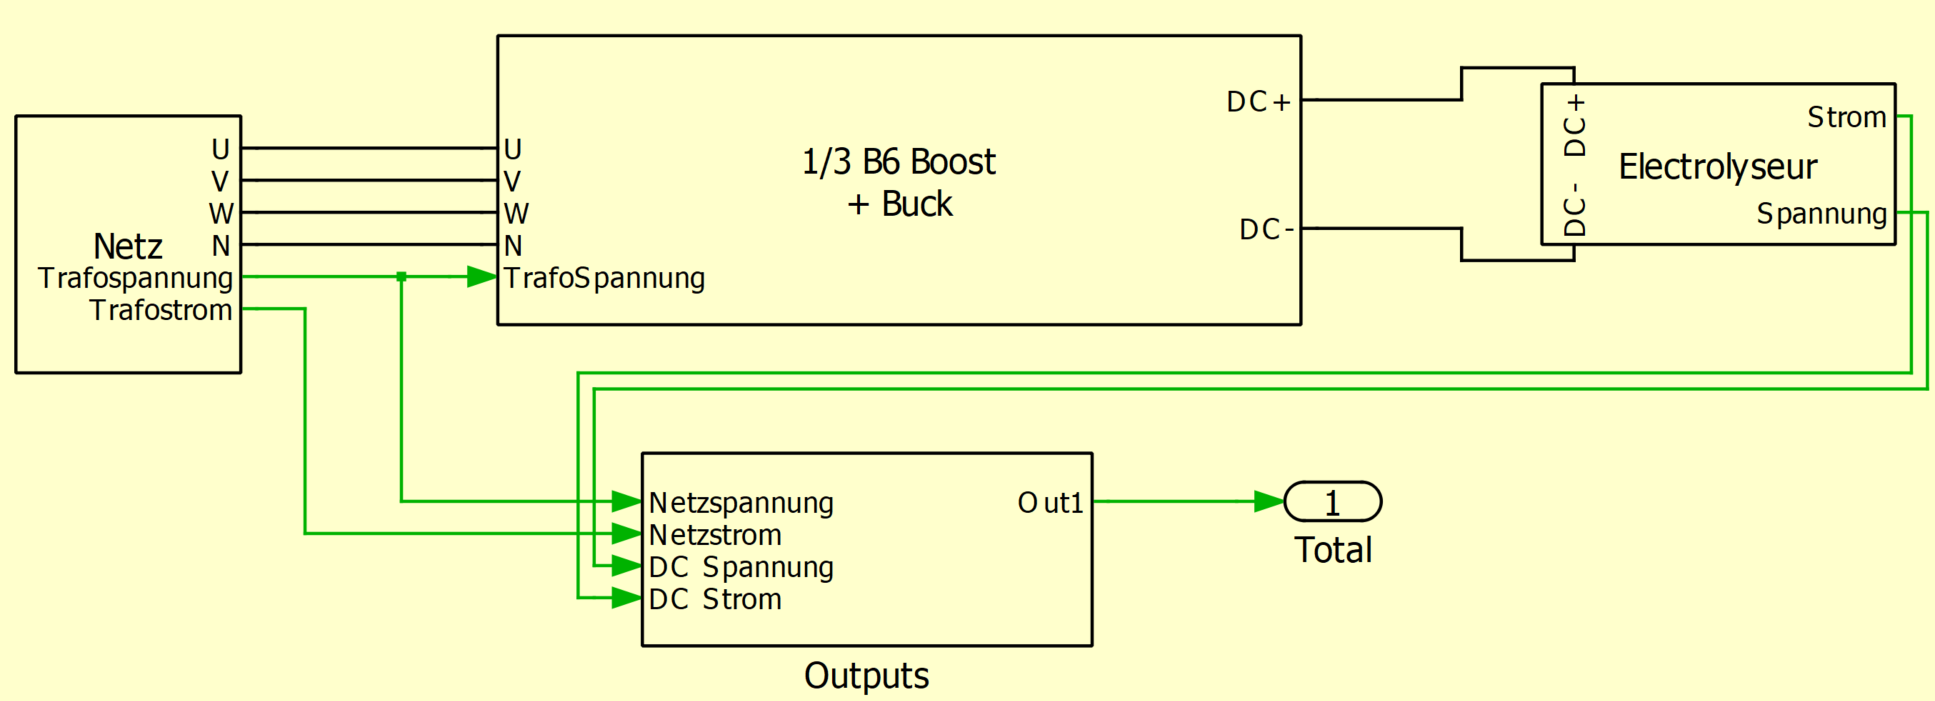
\includegraphics[width=0.9\linewidth]{content/Grafiken/PLECS_Simulationsaufbau}
\caption[Übersicht der PLECS Simulation]{Übersicht der PLECS Simulation}
\label{fig:plecssimulationsaufbau}
\end{figure}
Das Netz wird durch eine einfache Drehstromquelle dargestellt und kann in späteren schritten durch Netzimpedanzen und Fehlerszenarien ergänzt werden. Der Elektrolyseur besteht zur Vereinfachung aus einem passenden Lastwiderstand, der die entsprechend dem Skript eingestellte Leistung im Betriebspunkt abruft. Außerdem werden einige Widerstände eingesetzt, um \gls{PLECS} die Berechnung zu ermöglichen, da sonst im Einschaltvorgang durch Kapazitäten unendlich hohe Ströme entstehen würden und im realen Aufbau immer parasitäre Widerstände vorhanden sind.
\begin{figure}
\centering
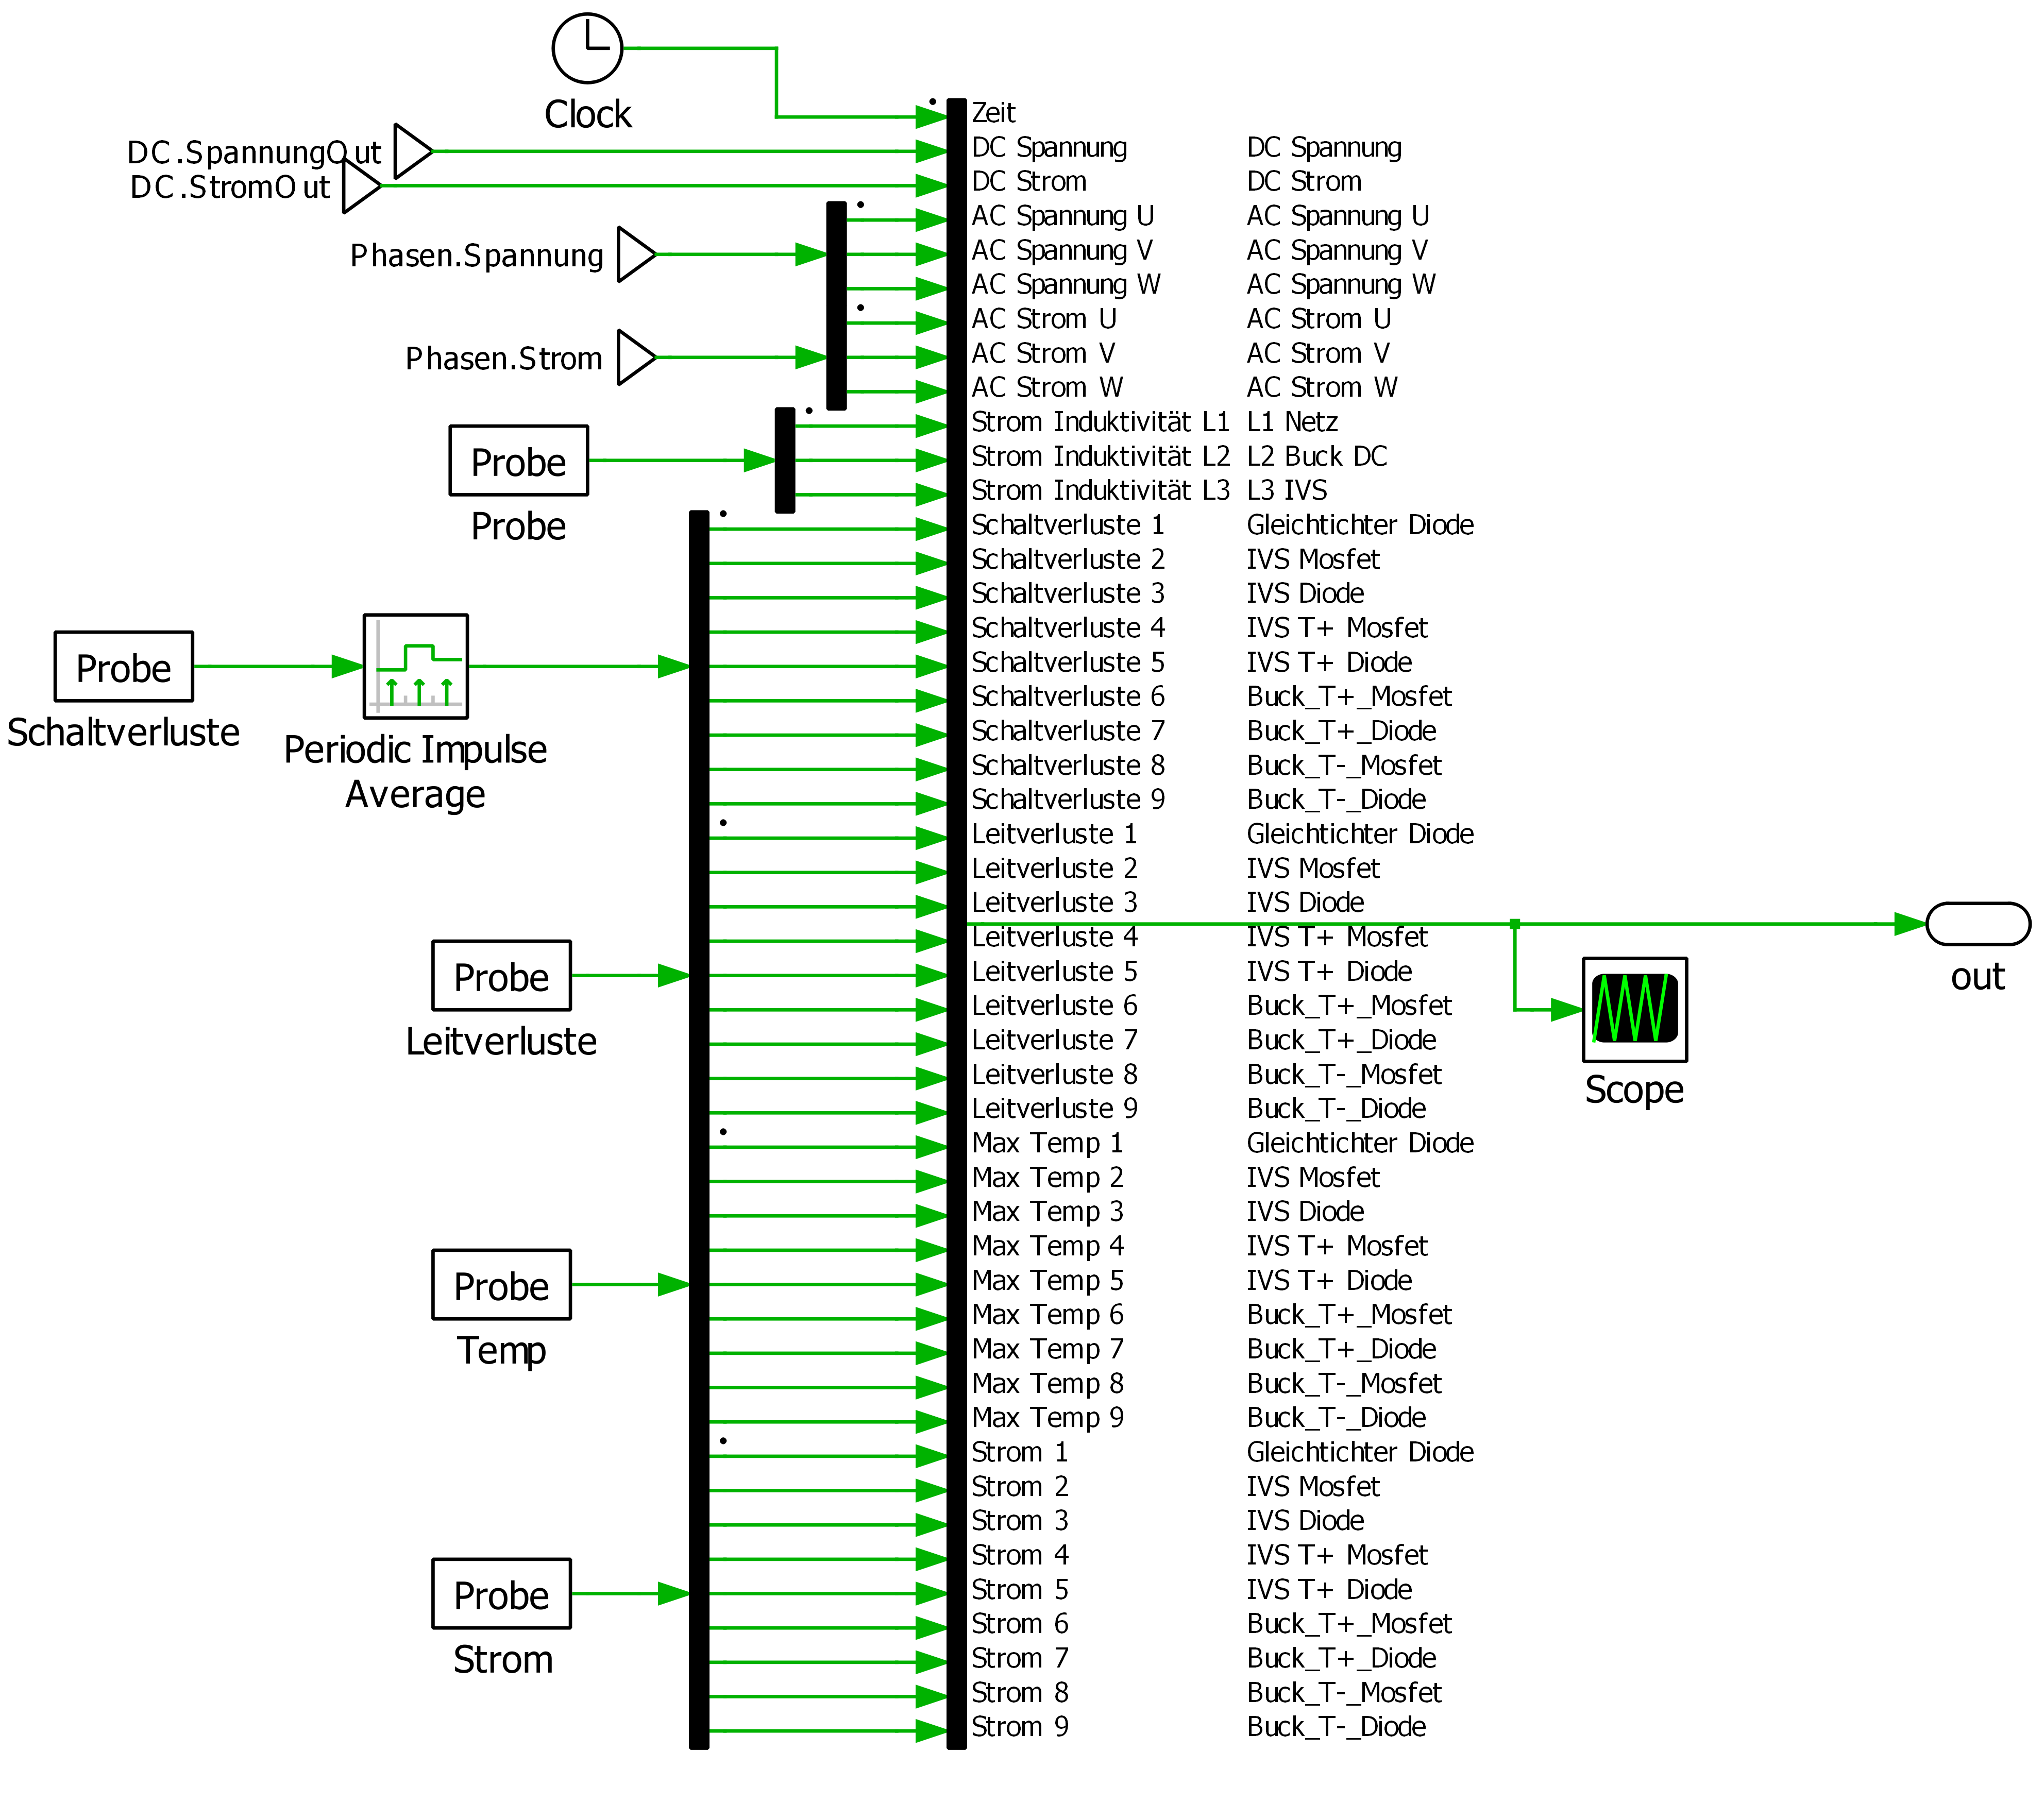
\includegraphics[width=0.9\linewidth]{content/Grafiken/Plecs_Out}
\caption[Zusammenfassung der Simulationsoutputs]{Zusammenfassung der Simulationsoutputs}
\label{fig:plecsout}
\end{figure}


\section{Randbedingungen}
Für den Gleichrichter werden Grundlegende Parameter festgelegt um die Auslegung für die Simulation durchführen zu können. Die Spannungsschwankung am Eingang wird auf 10 \% begrenzt, dies kann durch Varistoren oder ähnliches in der späteren Anwendung sichergestellt werden.

\begin{itemize}
\item Ausgangsleistung: 200 kW
\item Ausgangsspannung: 482-680 V
\item Ausgangsstrom: 	295 A
\item \gls{Ull}:		617 V
\item Netzfrequenz		50 Hz
\item Filterblindleistung: 3 \%
\item Schaltfrequenz: 20 kHz
\item Netzspannungsschwankung: 10 \%
\end{itemize}

Die Regelungen werden in den Simulationen nur im ein geschwungenen Zustand betrachtet, da dies für den Vergleich in festen Betriebspunkten ausreicht. Dies erleichtert die Auslegung der Regler, die Parameter werden so gewählt, dass ein stabiler Zustand erreicht wird und keine Oszillationen oder ähnliches Auftreten. Außerdem wird für die Bewertung die letzte Periode der Simulation verwendet, dieser Abschnitt wird zur späteren Betrachtung gespeichert.

\section{Tiefsetzsteller}
	Der Tiefsetzsteller kann in den beiden Schaltungen entkoppelt betrachtet werden, für die Auslegung der Induktivität ist dies von Vorteil. Die Reglung kann ebenso entkoppelt erfolgen und ermöglicht somit eine getrennte Stabilitätsbetrachtung und Optimierung. 
	\subsection{Auslegung der Induktivität}
	Die Speicherdrossel wird anhand von Formel \ref{eq:BuckL} ausgelegt, dabei liegt die Netzspannung bei maximal $U_{LLmaxPeak}=1,1 \cdot 617 \si{\V} \cdot \sqrt{2}=959,8 \si{\V}$ und die Ausgangsspannung bei mindestens 482 \si{\V}. Daraus ergeben sich die maximalen Parameter, die der Tiefsetzsteller umsetzen muss. Es ergibt sich somit eine Induktivität von 134,16 \si{\micro \henry}, siehe Formel \ref{eq:BuckLwert}. Die Energie beträgt 7,78 Joule, bei einem Ausgangsstrom von 294 A. 
	\begin{equation}
	\label{eq:BuckLwert}
	L_{T}=\dfrac{959,8\si{\V} - 482 \si{\V}}{20 \si{\kilo \hertz}\cdot 0,3 \cdot 295 \si{\ampere}}\cdot \dfrac{482 \si{\V}}{969,8 \si{\V}}= 134,16 \si{\micro \henry} 
	\end{equation}
	\begin{equation}
		E=0,5 \cdot L_{T} \cdot I^{2} = 7,78 J
	\end{equation}
	\subsection{Regelung}
	Die Regelung lässt sich anhand der in Abschnitt \ref{sec:Buck} beschrieben Zusammenhänge der Eingangsspannung auslegen, der Dutycycle \gls{D} ist das Verhältnis aus Eingangs- und Ausgangsspannung. Aufgrund der sechspulsigen Zwischenkreisspannung schwankt der Dutycycle \gls{D} leicht aber da eine feste Ausgangsspannung gewünscht ist, lässt sich die Regelung durch einen PI-Regler implementieren. 


\section{IAF}
	Der Hauptteil der Simulation liegt in den Leistungshalbleitern, deren Anordnung kann in Abb. \ref{fig:iafplecsmain} und \ref{fig:iafplecsivs} gefunden werden. Für die Verlustleistungsbestimmung werden Modelle von Infineon verwendet, für die Dioden und den \gls{IVS} wird ein gemeinsames Modul vorgesehen mit 5 \si{\milli \ohm} \gls{SiC} \gls{MOSFET}. Die Halbbrücke an der Induktivität wird aus einem Modul mit einem Nominalstrom von 45 A umgesetzt. Alle Halbleiter haben eine Spannungsfestigkeit von 1200 V.
	\begin{figure}
		\centering
		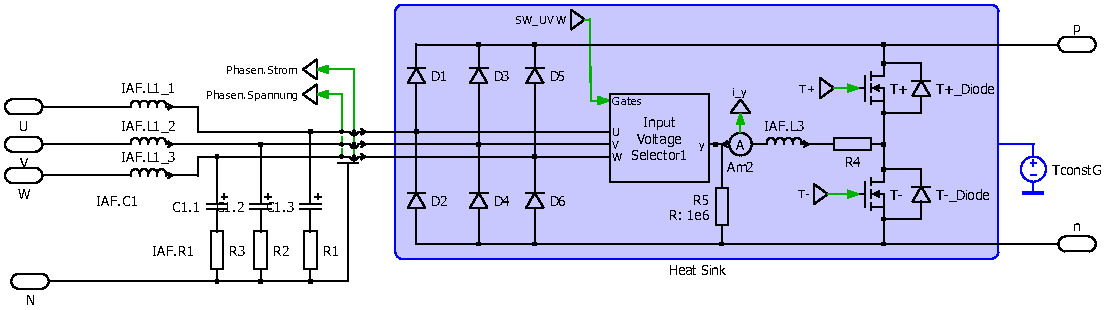
\includegraphics[width=1\linewidth]{content/Grafiken/IAF_Plecs_main}
		\caption{Simulationsaufbau der Halbleiter des IAF}
		\label{fig:iafplecsmain}
	\end{figure}
	\begin{figure}
		\centering
		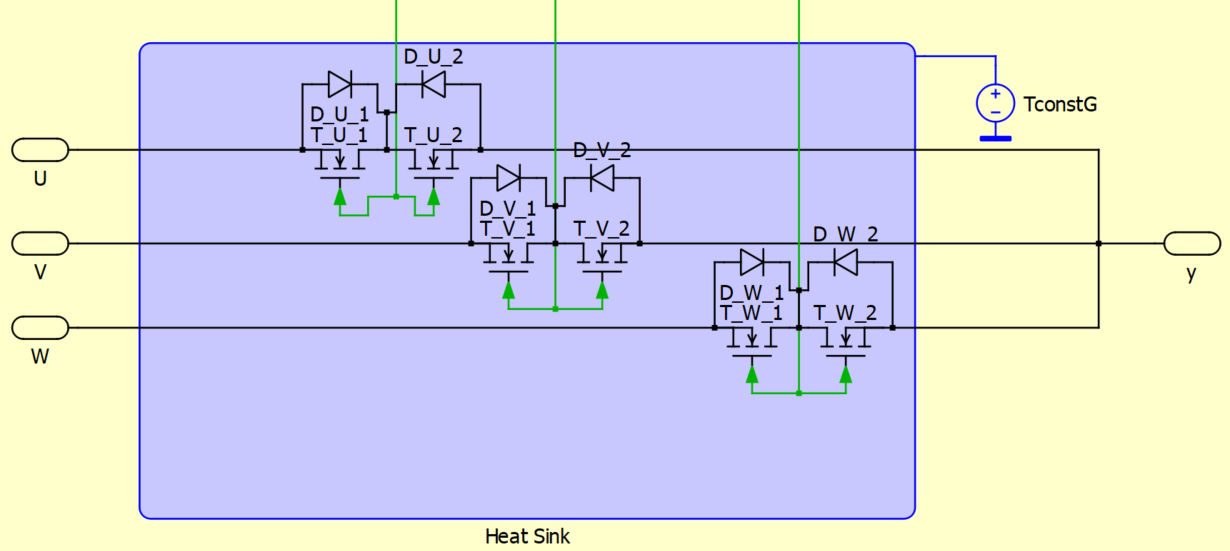
\includegraphics[width=0.9\linewidth]{content/Grafiken/IAF_Plecs_IVS}
		\caption{Simulationsaufbau der Halbleiter des IVS vom IAF}
		\label{fig:iafplecsivs}
	\end{figure}
	
	\cite{IAF99}
	
	\subsection{Auslegung der Induktivitäten}
		Der maximale Stromrippel ergibt sich aus der Leistung und der minimalen Netzspannung und beträgt 44,1 \si{\A}, siehe Formel \ref{eq:DeltaIIVS}. Der Rippelstrom wird wieder auf 30\% des Nominalstroms ausgelegt. Somit muss die Induktivität einen Wert von 272\si{\micro \henry} besitzen, siehe Formel \ref{eq:Livs}.  
		
		\begin{equation}
		\label{eq:DeltaIIVS}
		I_{\Delta max IVS}= \dfrac{0,3\cdot \sqrt{2} \cdot 200 \si{\kilo \watt}}{2 \cdot \sqrt{3} \cdot 617 \si{V} \cdot 0,9} = 44,1 \si{\A}
		\end{equation}
		
		\begin{equation}
			\label{eq:Livs}
			L_{IVS}= \dfrac{U_{LLmaxPeak}}{4\cdot f \cdot I_{\Delta max IVS}} = 272 uH
		\end{equation}
		Bei der Betrachtung der Energie muss berücksichtigt werden, dass der Strom in der Drossel bei Blindleistung steigt und somit die Energie im quadratischen Verhältnis steigt. Der Strom bei einer Phasenverschiebung von 30 Grad wird über den Faktor $sin(30)=0,5$ berechnet und ergibt sich somit zu 132,33 A, siehe Formel \ref{eq:IAF_I30}.
		\begin{equation}
			\label{eq:IAF_I30}
			I_{IAF30°}=\dfrac{0,5\cdot \sqrt{2} \cdot 200 \si{\kilo \watt}} { \sqrt{3} \cdot 617 \si{V}} = 132,33 \si{\A}
		\end{equation}
		 Die Energie in der Drossel und damit relevante Größe für die Bewertung beträgt 2,38 Joule, siehe Formel \ref{eq:EL_IVS}.
		\begin{equation}
			\label{eq:EL_IVS}
			E_{IVS}=0,5 \cdot L_{IVS} \cdot I_{\Delta max IVS}^{2} = 2,38 J
		\end{equation}
		Außerdem wird eingangsseitig eine Filterinduktivität mit dem Wert 1 \si{\micro \henry} eingesetzt, diese hat eine gespeicherte Energie von 0,1 Joule, siehe Formel \ref{eq:E_IAF_ACL}. Aufgrund der Dreiphasigen Anwendung, wird der Wert direkt mit dem Faktor drei multipliziert.
			\begin{equation}
			\label{eq:E_IAF_ACL}
			E_{L_IAF_AC}=3\cdot 0,5 \cdot 1 \si{\micro \henry} \cdot (260 \si{\ampere})^{2} = 0,1 J
		\end{equation}
	
	\subsection{Regelung}
		Der Tiefsetzsteller wird durch einen PI Regler für die Fehlerkorrektur angesteuert, der ideale Tastgrad wird anhand der gewünschten Ausgangsspannung, welche über den Sollstrom und bekannten Lastwiderstand generiert wird, und der Zwischenkreisspannung \gls{Upn} bestimmt. Der Tastgrad wird dann in einen PWM-Generator gegeben, welcher das Signal mit der gewünschten Schaltfrequenz von 20 kHz generiert. Um die Schaltverluste und insbesondere Leitverluste beim kommutieren in den Dioden zu berücksichtigen wird eine Totzeit von 500 \si{\nano \second} eingestellt, vgl. Abb. \ref{fig:iafbuckcontrol}.
		\begin{figure}[H]
			\centering
			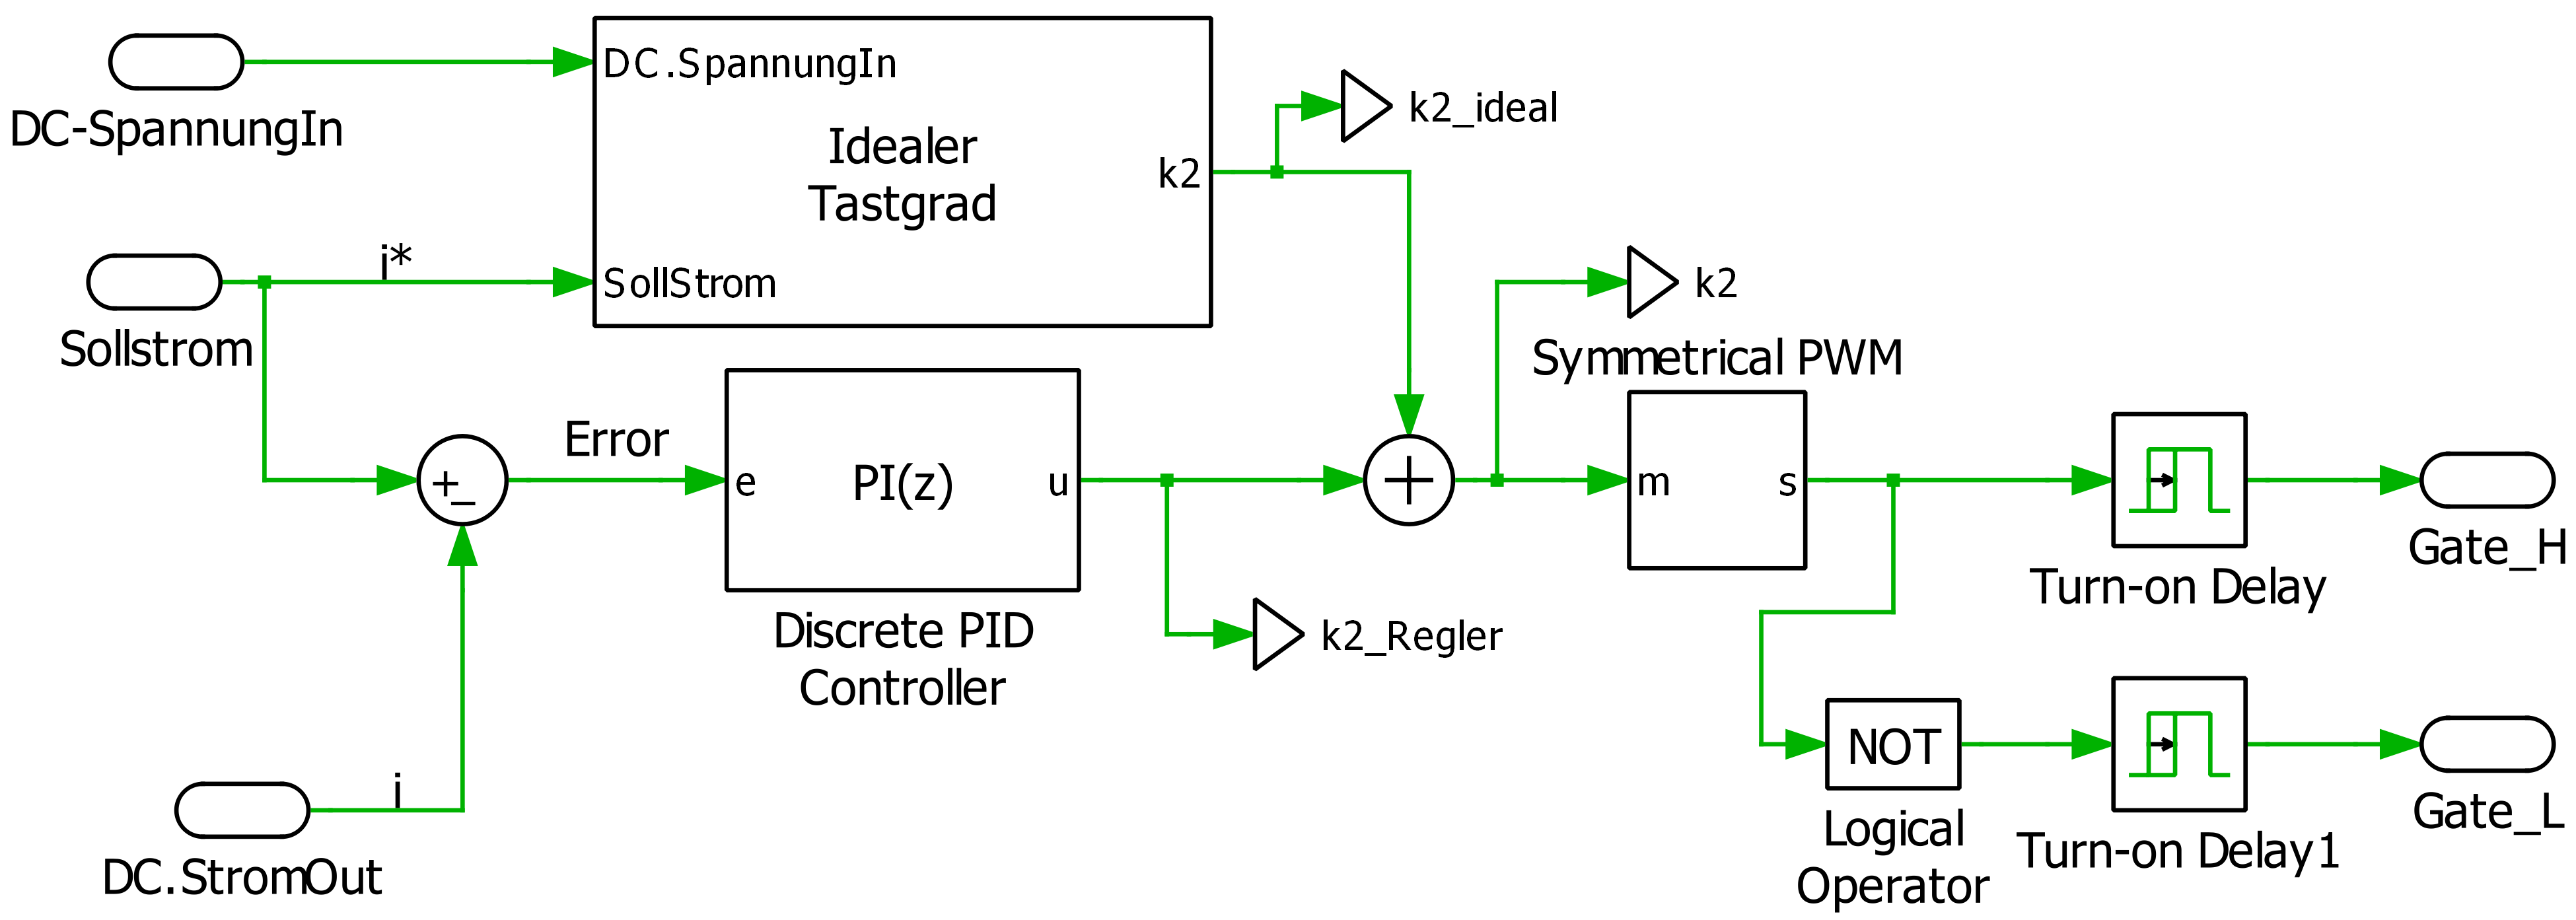
\includegraphics[width=0.9\linewidth]{content/Grafiken/IAF_BuckControl}
			\caption{Regelung des Tiefsetzstellers des IAF}
			\label{fig:iafbuckcontrol}
		\end{figure}
		
		Die Regelung des \gls{IVS} Stroms wird anhand der Struktur von Soeiro et al. umgesetzt, siehe Abb. \ref{fig:iafpapercontrol} \cite{Soeiro.2013}. 
		 \begin{figure}[H]
			\centering
			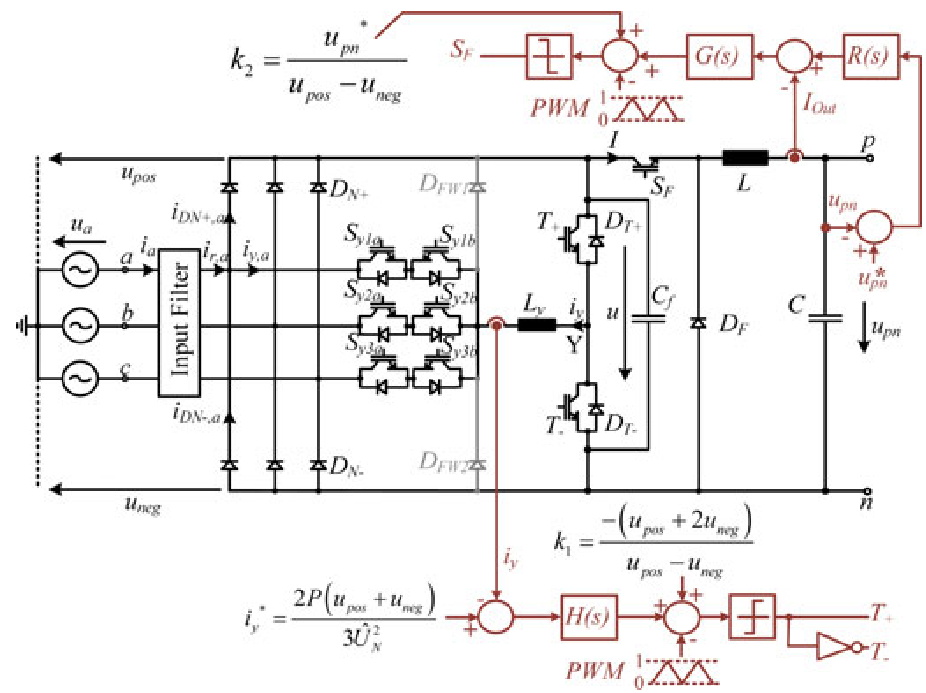
\includegraphics[width=0.7\linewidth]{content/Grafiken/IAF_Paper_Control}
			\caption{Struktur der Regelung des IAF \cite{Soeiro.2013}}
			\label{fig:iafpapercontrol}
		\end{figure}
		Die Umschaltung zwischen den Phasen wird über eine von \gls{PLECS} vorhandene \gls{PLL} zur Winkelbestimmung und anschließende Sektorbestimmung anhand des Winkels umgesetzt. Die Auswahl der entsprechenden Schalter wird über ein C-Skript implementiert, siehe Abb. \ref{fig:plecsiafivscontrol}. 
		\begin{figure}[H]
			\centering
			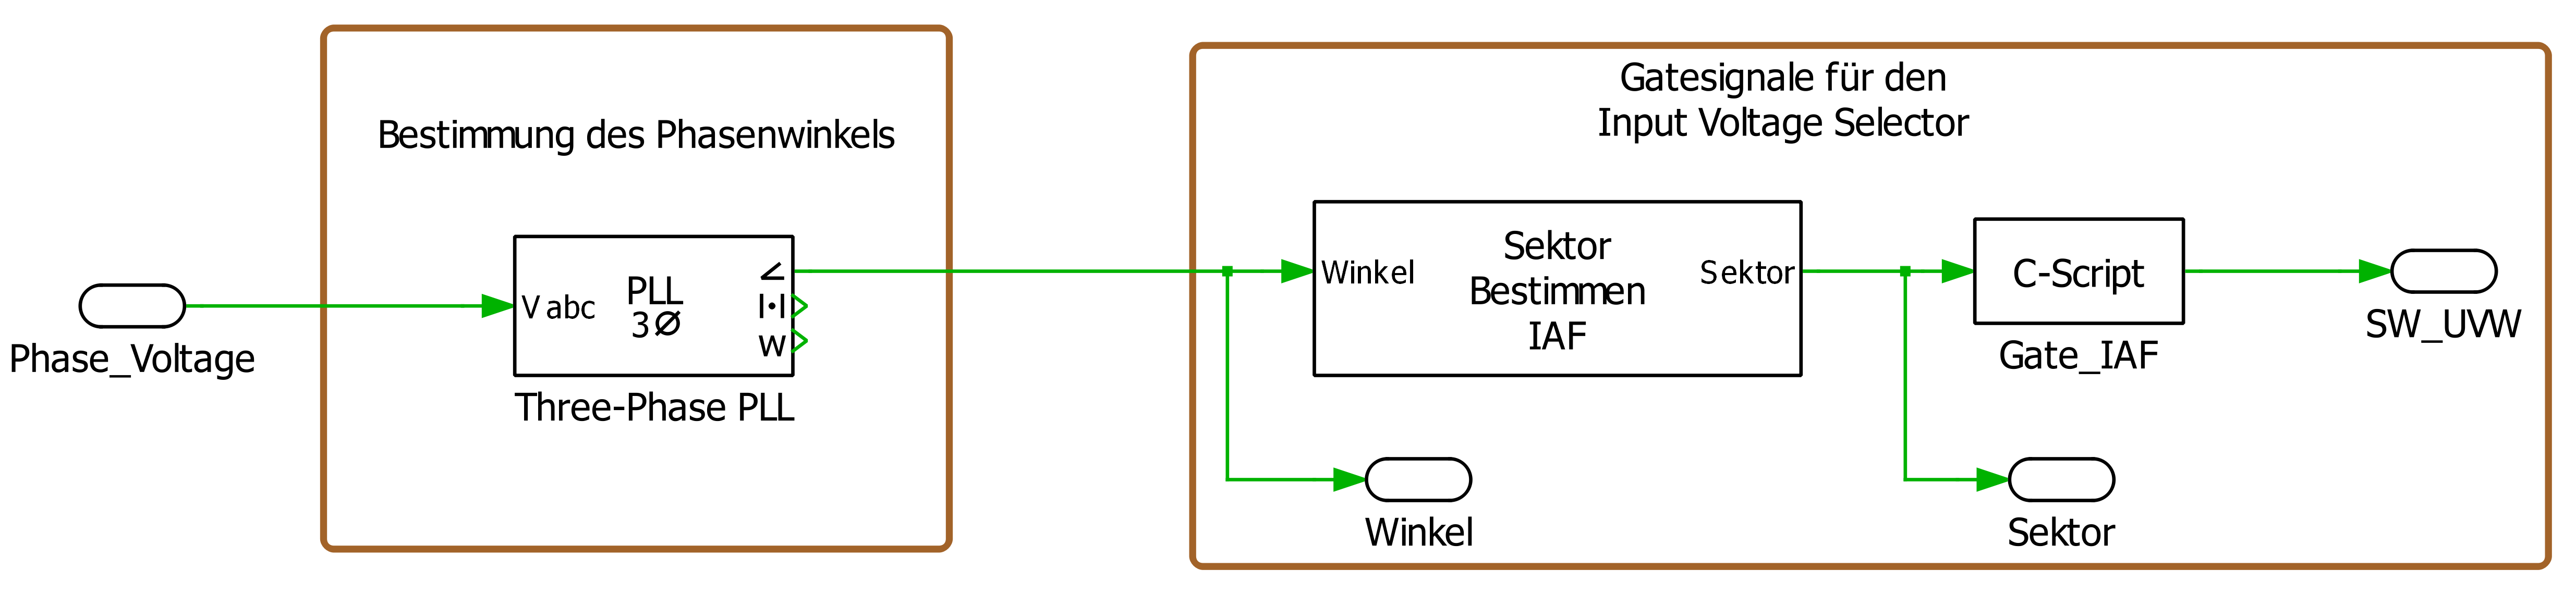
\includegraphics[width=1\linewidth]{content/Grafiken/PlecsIAFivscontrol}
			\caption{PLECS Aufbau der \gls{IVS} Ansteuerung}
			\label{fig:plecsiafivscontrol}
		\end{figure}
		Über die Spannungen und Ausgangsleistung kann der soll Strom, welcher durch den\gls{IVS} eingeprägt werden soll bestimmt werden, siehe Abb. \ref{fig:plecsiafivsi}.
		\begin{figure}
			\centering
			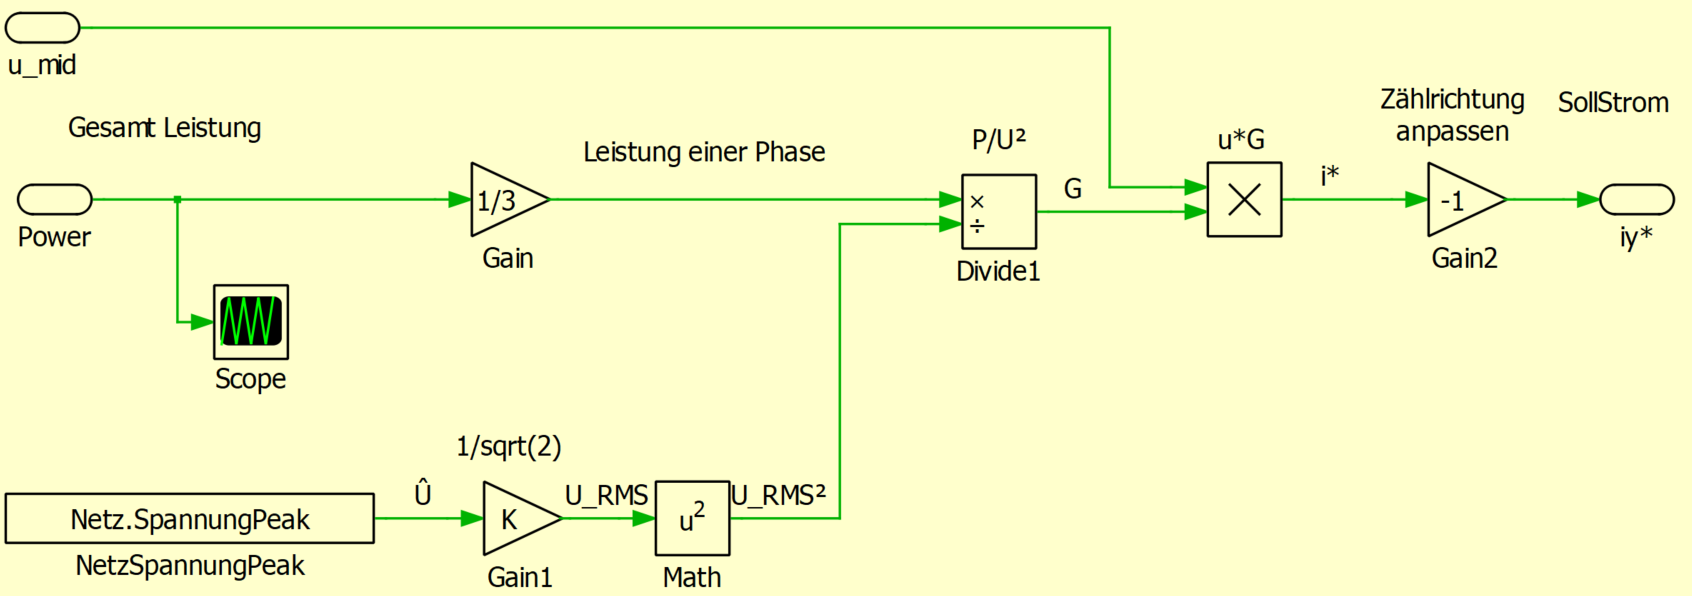
\includegraphics[width=1\linewidth]{content/Grafiken/PlecsIAFivsI}
			\caption{Bestimmung des soll Stroms im IVS Pfad}
			\label{fig:plecsiafivsi}
			
		\end{figure}
		Der ideale Tastgrad K1 wird über das Verhältnis der Spannungen durch den formelmäßigen Zusammenhang in Gleichung \ref{eq:K1} bestimmt. Die Regelung des Stroms wird über einen diskreten PI Regler Block aus der PLECS Bibliothek implementiert. Die Signale zur Gateansteuerung werden über einen PWM Generator erzeugt und anschließend zur Totzeit Implementierung durch eine Einschaltverzögerung verzögert. Dieser Aufbau kann in Abb. \ref{fig:plecsiafivsk1}.
		
		\begin{equation}
			\label{eq:K1}
			K1 = \dfrac{U_{mid}- U_{low}}{U_{high} -U_{low}} 
		\end{equation}
		
		\begin{figure}
			\centering
			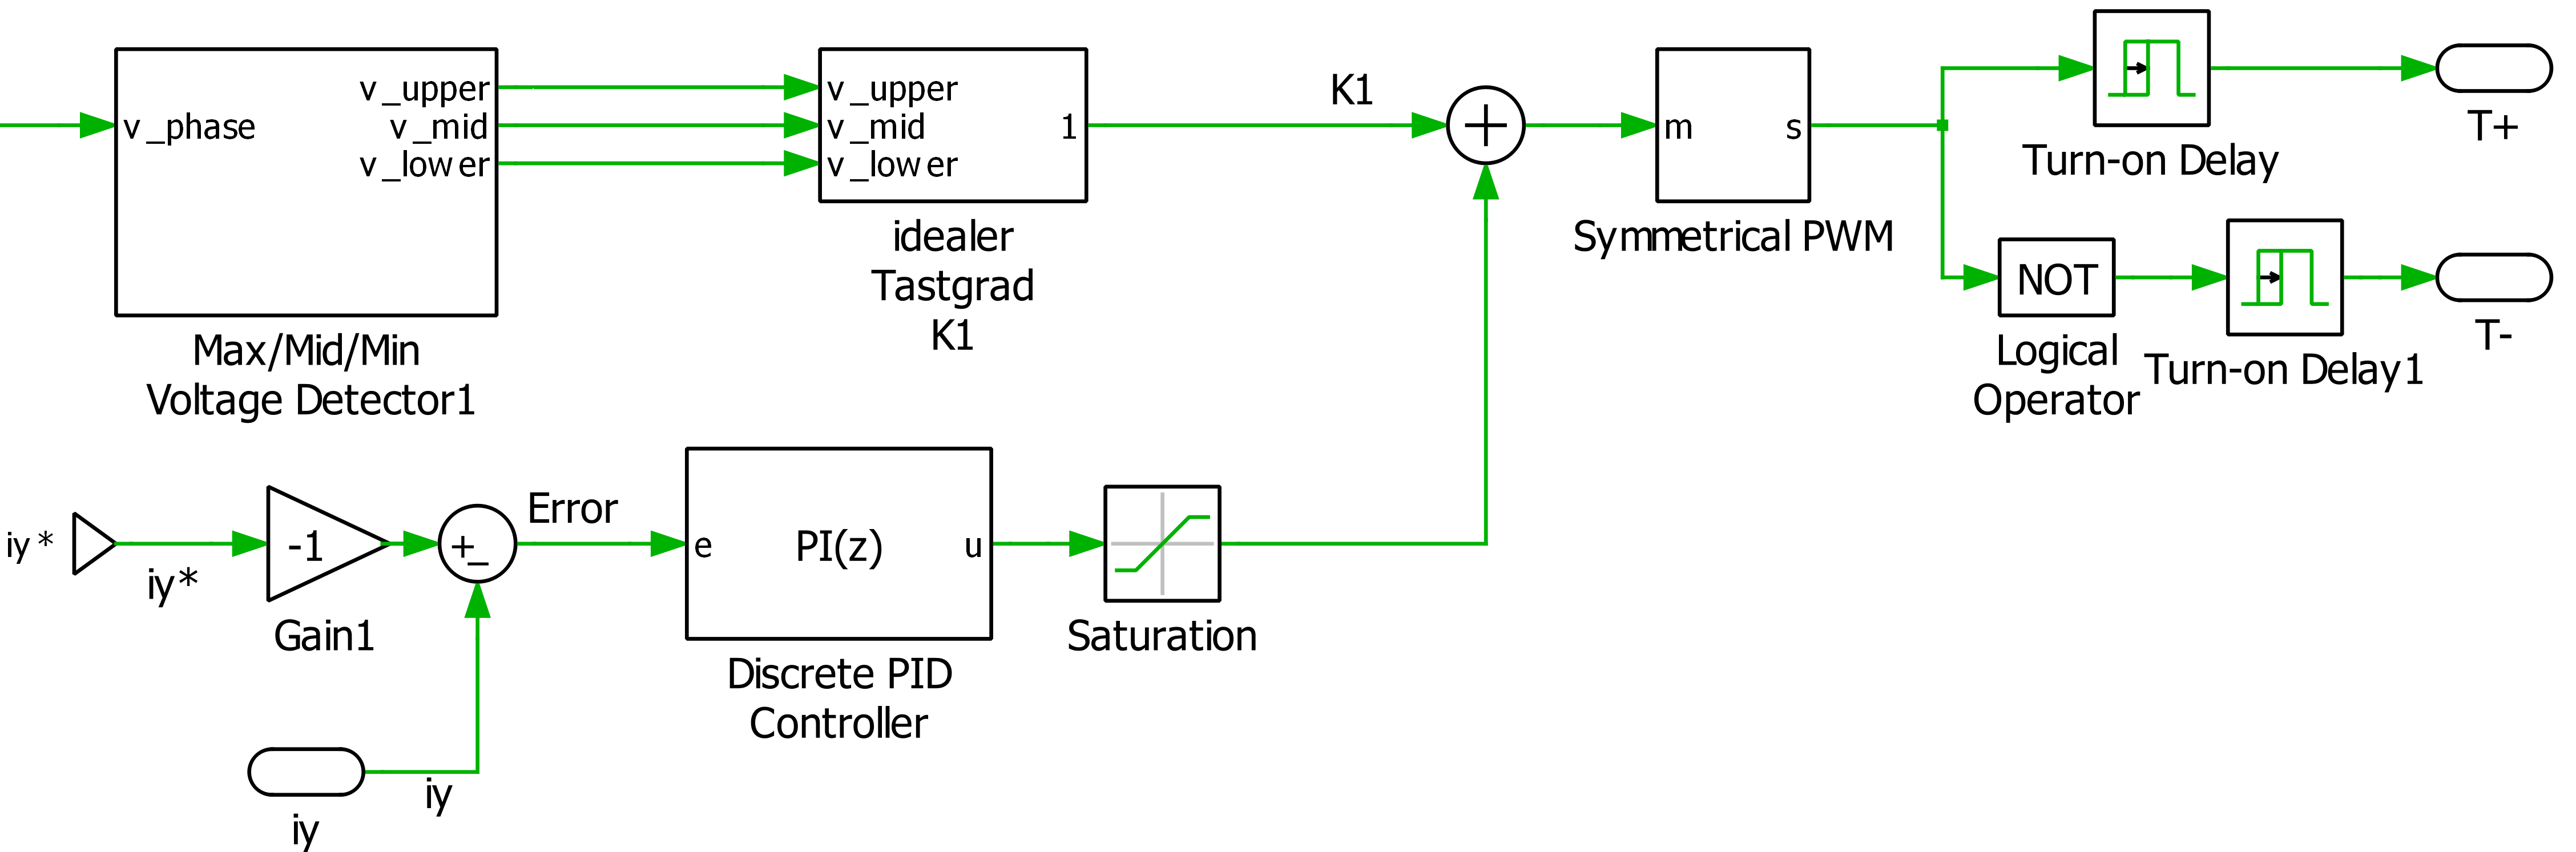
\includegraphics[width=1\linewidth]{content/Grafiken/PlecsIAFivsK1}
			\caption{Regelung des Stroms in der mittleren Phase}
			\label{fig:plecsiafivsk1}
		\end{figure}
		
	

\section{B6 1/3 PFC Buck}
Die in Kapitel \ref{sec:GrundlagenB6} dargestellte Schaltung wird durch Halbbrücken Module des Typs FF2MR12W3M1H\_B11 von Infineon implementiert. Dabei handelt es sich um verbreitete 1200 \si{\volt} Module, sie besitzen einen nominellen Einschaltwiderstand von etwa 2 \si{\milli \ohm} und können Spitzenströme von bis zu 800 \si{\ampere} schalten \cite{IFAGFF2}. Um die Ausgangsleistung auch bei geringerer Spannung bereitstellen zu können und ein späteres Interleaving zu ermöglichen werden für den Tiefsetzsteller zwei Halbbrücken vorgesehen.

		\subsection{Auslegung der Netzinduktivität}
			Aufgrund der Limitierung des Eingangsstroms zur effizienten Auslegung der Drossel, wird die Ausgangsleistung bei Blindleistungsbereitstellung reduziert. Dies ist wie bereits in \ref{sec:AnfStromnetz} erläutert durch den Netzbetreiber gestattet. Der Rippelstrom in der Drossel wird wie gehabt auf 30 \% des Effektivstroms ausgelegt, welcher bei Spannungseinbruch auf 90 \% am höchsten ist. Der Rippelstrom beträgt somit 88,2 Ampere, siehe Formel \ref{eq:DeltaI_B6}.\\
			
			\begin{equation}
				\label{eq:DeltaI_B6}
				I_{\Delta max B6}= \dfrac{0,3\cdot \sqrt{2} \cdot 200 \si{\kilo \watt}}{\sqrt{3} \cdot 617 \si{V} \cdot 0,9} = 88,2 \si{\A}
			\end{equation}
			Die Induktivität kann durch den gleichen Zusammenhang wie beim \gls{IAF} \gls{IVS} ausgelegt werden und beträgt 136 \si{\micro \henry}, siehe Formel \ref{eq:L_B6}.
			\begin{equation}
				\label{eq:L_B6}
				L_{B6}= \dfrac{U_{LLmaxPeak}}{4\cdot f \cdot I_{\Delta max B6}} = 136 uH
			\end{equation}
			Die gespeicherte Energie in der Induktivität wird ebenfalls über den Zusammenhang der Netzspannung und Ausgangsleistung definiert, erhöht sich jedoch nicht durch Blindleistungsbereitstellung. Die gespeicherte Energie pro Phase ergibt 4,76 Joule nach Formel \ref{eq:EL_B6} und muss aufgrund der Dreiphasigen Ausführung wieder dreifach gewertet werden. Somit ergibt sich eine Gesamtenergie für die Hauptinduktivität der Topologie von 14,28 Joule.
			
			\begin{equation}
			\label{eq:EL_B6}
			E_{LB6}=0,5 \cdot L_{B6} \cdot {\dfrac{\sqrt{2} \cdot 200 \si{\kilo \watt} }{\sqrt{3} \cdot 617 V}}^{2} = 4,76 J
			\end{equation}
			
			

		
		\subsection{Regelung}
			Die Regelung besteht aus einer Kaskadierten Struktur mit vier Stufen. Die erste ist die Ausgangsspannungsregelung, welche durch die Sollleistung und Netzspannung die gewünschte äquivalente Phasenimpedanz als Eingangsgröße für die Phasenstromregelung bildet.\\
			In der dritten Stufe wird die Phase mit der mittleren Spannung ausgewählt und die Zwischenkreisspannung \gls{Upn} anhand der Phasenlage bestimmt. Die Zwischenkreisspannung resultiert als sechspulsige Gleichspannung und dient als Eingangsspannung für den Tiefsetzsteller. Die mittlere Phasenspannung wird als Referenz für den Tastgrad der entsprechenden Halbbrücke verwendet und prägt somit einen zur Spannung proportionalen Strom ein. Somit wird immer nur eine der drei Halbbrücken getaktet geschaltet, die anderen beiden sind wie bei einem Diodengleichrichter auf die jeweils positivste und negativste Spannung geschaltet.\\
			Die vierte Stufe ist die des Tiefsetzstellers, mit Reglern für den Eingangsstrom sowie die Ausgangsspannung.
			
			\begin{figure}
			\centering
			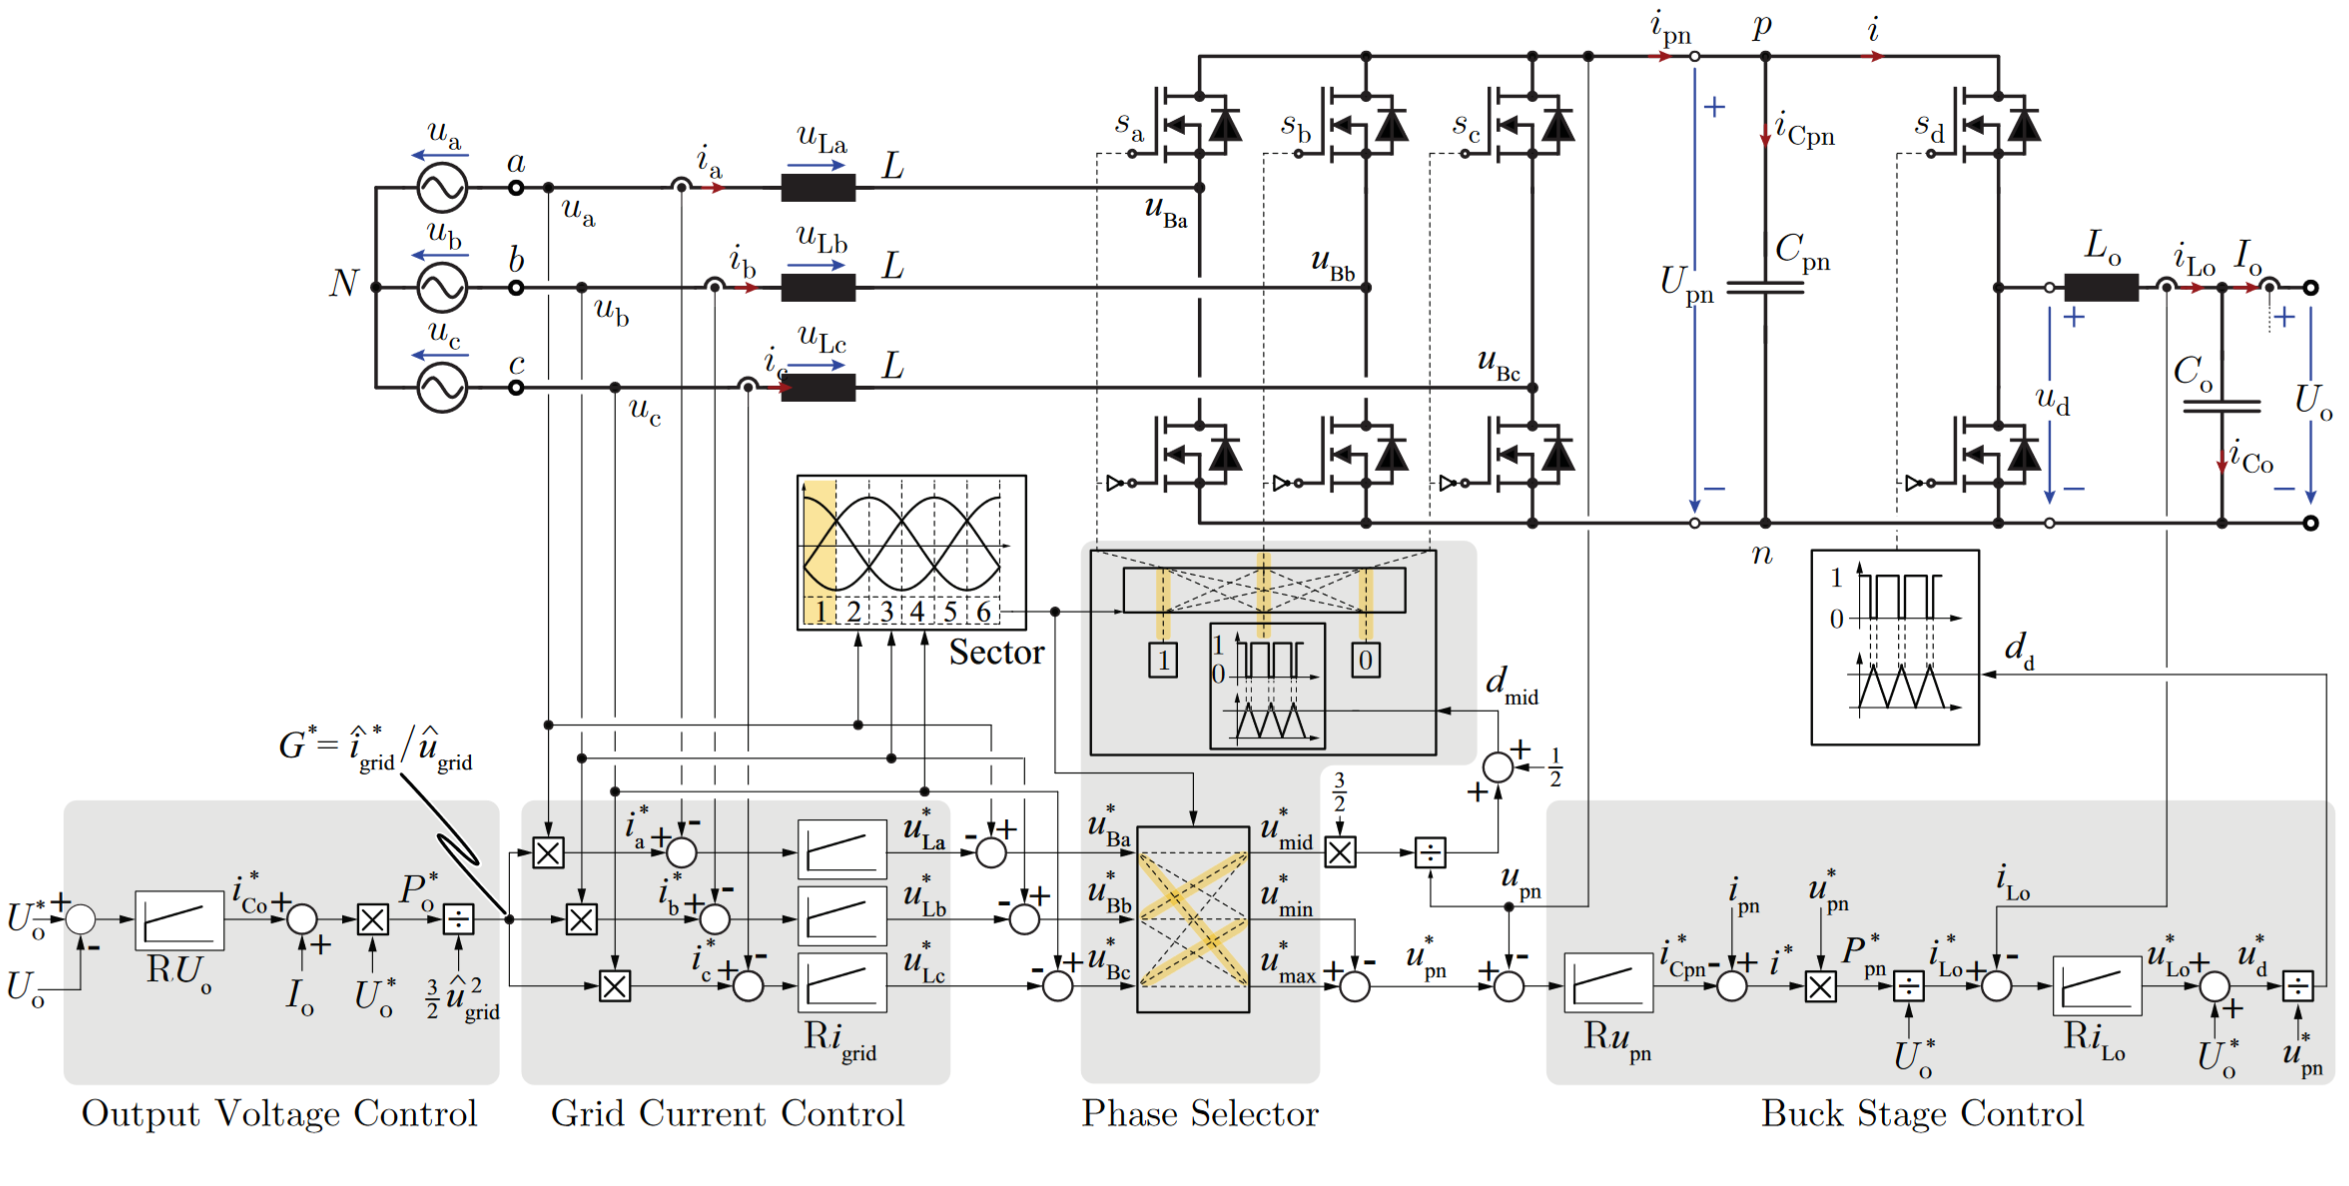
\includegraphics[width=0.9\linewidth]{content/Grafiken/B6-Control-orig}
			\caption[Regelung des \gls{B6PFC}]{Regelung des \gls{B6PFC} \cite{13PWMPFC}}
			\label{fig:b6-control-orig}
			\end{figure}
